\newpage
\section{Aufgabe 1}

\subsection{Aufgabenstellung}
Sie haben in den vorhergehenden Praktika eigene Verteilte Anwendungen entwickelt, die Sie nun analysieren sollen.\\\\Gehen Sie wie folgt vor:

\begin{enumerate}[label=(\alph*)]
	\item Starten Sie die Wireshark-Software auf Ihrem Rechner und machen Sie sich mit den Möglichkeiten der Aufzeichnung des Netzwerkverkehrs und der detaillierten Anzeige der aufgezeichneten Abläufe vertraut.
	\item Realisieren Sie einen Filter für die Aufzeichnung des Netzwerkverkehrs, mit dem nur noch Frames mit TCP Segmenten mit der Portnummer 8999 aufgezeichnet werden.
	\item Starten Sie nun den Datentransfer, den Sie im vergangenen Praktikum implementiert haben (wahlweise die UDP- oder TCP-Variante).\\Stoppen Sie die Aufzeichnung sofort, wenn Client und Server beendet sind.
	\item Analysieren Sie die ausgetauschten Nachrichten zwischen Client und Server. An welcher Stelle finden Sie die Response vom Servers? Welche Nachrichten werden beim Verbindungsaufbau und -abbau ausgetauscht?
\end{enumerate}

\subsection{Vorbereitung}
Um diese Aufgabe lösen zu können muss man die vorherige Aufgabe gelöst haben und sich mit Wireshark auseinandersetzen.

\subsection{Durchführung}

\subsubsection{a)}
Da wir unter MacOS arbeiten, haben wir keine Möglichkeit gefunden um uns den sogenannten \textit{Capture Info Dialog} nicht anzeigen lassen, da das entfernen des Harken nichts geändert hat. Sonst wurde die komplette Kurzanleitung durchgearbeitet.
\begin{figure}[H]
	\centering
	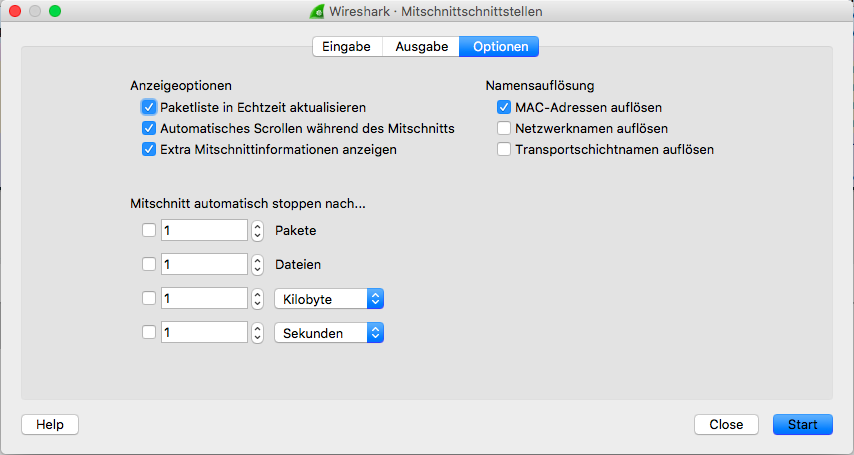
\includegraphics[width=0.8 \linewidth]{images/w01}
	\caption{Capture Options} \label{ordner}
\end{figure} 
Man kann sich aber unter den Statistiken die bei der Aufzeichnung aufgezeichneten Pakete den prozentualen Anteil der Protokolle anzeigen lassen.
\begin{figure}[H]
	\centering
	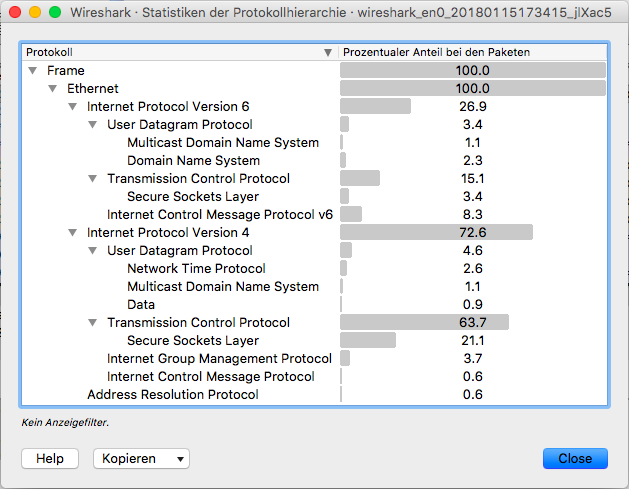
\includegraphics[width=0.7 \linewidth]{images/w02}
	\caption{Protokollhierachie} \label{ordner}
\end{figure} 

\subsubsection{b)}
Für diese Aufgabe erstellen wir einen sogenannten \textit{Mitschnittfilter}, dies geht unter \textbf{Aufzeichnen > Mitschnittfilter}. Um die Aufzeichnung nun damit zu starten wählt man diesen bei der Auszeichnung aus. 
\begin{figure}[H]
	\begin{minipage}[b]{.5 \linewidth}
		\centering
		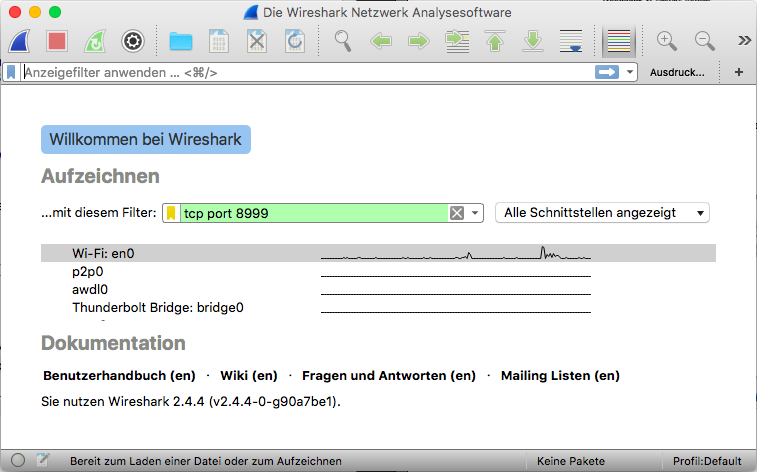
\includegraphics[width=.95 \linewidth]{images/w03}
	\end{minipage}
	\begin{minipage}[b]{.5 \linewidth}
		\centering
		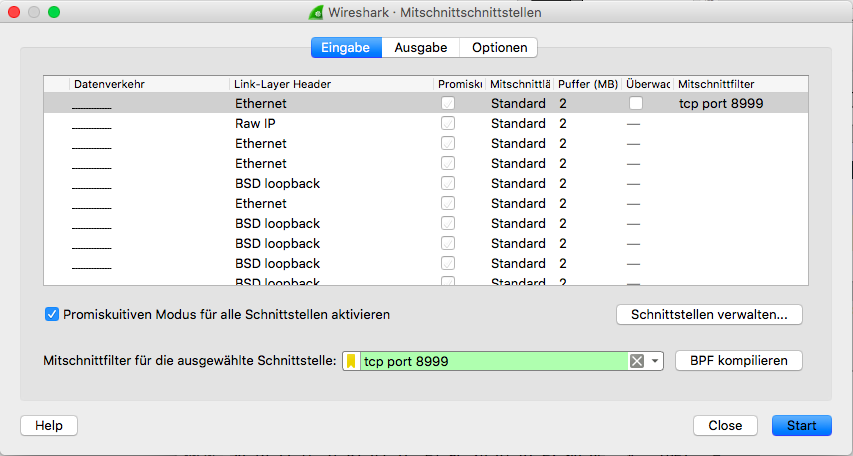
\includegraphics[width=.95 \linewidth]{images/w04}
	\end{minipage}
	\caption{Einstellung des Mitschnittfilters}
\end{figure}

\subsubsection{c)}
Wir nutzen für diese Aufgabe das Programm welches über das UDP-Protokoll arbeitet, da wir aber lokal arbeiten müssen wir über einen sogenannten \textit{Loopback} arbeiten.
\begin{figure}[H]
	\centering
	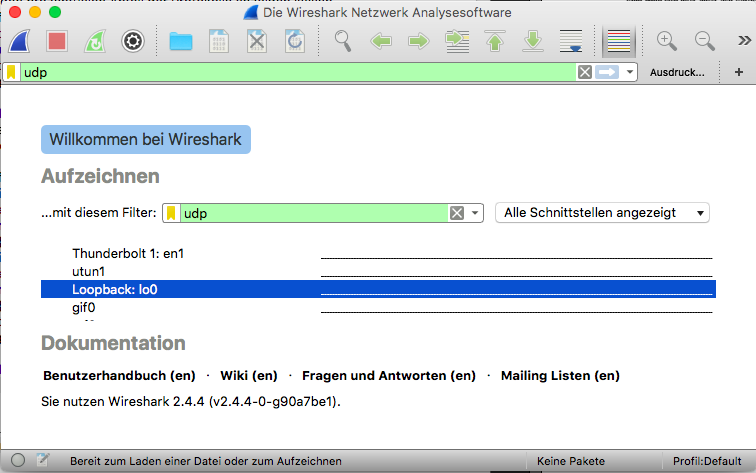
\includegraphics[width=0.7 \linewidth]{images/w05}
	\caption{Loopback} \label{ordner}
\end{figure} 

\subsubsection{d)}

